 % -*- encoding: UTF8 -*-
%
%%*****************************************************************************
%%									                         			Einführung									 
%%*****************************************************************************

\chapter{Introduction}
\label{Ch:Introduction}
%%*****************************************************************************


\section{Motivation}
The aging of our society is encouraging an institutional effort towards the early detection of diseases \cite{Fendrich2007}. As checkups and screenings become more common, there is a need for better, less invasive diagnostic methods that reduce the risks and discomfort to the patient. An example of a common invasive procedure is histology through biopsy, used in the diagnosis of possible cancerous lesions. When the tissue is located inside a lumen, this method involves identifying the area to be sampled by endoscopy, using forceps to extract a biopsy sample and performing the histology analysis \textit{ex situ}. 

A faster and less invasive alternative is optical biopsy: a collective name for advanced endomicroscopy methods allowing real-time, \textit{in-situ} diagnosis of tissue malignancies without the need of excision and histopathological analysis. Numerous techniques, such as endocytoscopy and fluorescence imaging, have already found their way into the clinical armamentarium over the last years; others, such as confocal laser endomicroscopy\cite{Jabbour2013}, Raman spectroscopy \cite{Bergholt2011} or optical coherence tomography (OCT)\cite{Park2012,Sun2011}, are expected to enter routine clinical use in the imminent future. Currently, none of these imaging modalities individually are yet to match the selectivity and specificity of traditional biopsy. This is why multi-modal imaging, which can provide complete tissue characterization through complementary modalities, will likely be the key to the success of optical biopsy.

The framework of this thesis aims to achieve optical biopsy through a compact endoscope with two imaging modalities: full field microscopy, which eases tissue identification, and OCT, which enables tomographic and volumetric imaging. The probe features a two-level design that integrates the two modalities, still allowing for independent optimization. 
Inside this framework, this thesis focuses on the OCT imaging device, implemented as a fiber scanner.

The next sections introduce the state of the art of endoscopic OCT and multimodal probes followed by a summary of the key results.

\section{State of the Art}
This section summarizes the technologies that paved the way towards the multimodal endoscopic probe developed in this project: OCT and multimodal endoscopy.

Shortly after the development of OCT technology \cite{Huang1991}, the first medical applications were reported, finding a niche in ophthalmology. But its optical sectioning abilities, allowing imaging with resolutions in tens of micrometers as seen in the example from \autoref{fig:OCTretina}, moved soon from bench-top ophthalmology systems to endoscopic probes.  
\begin{figure}[h!]\centering
      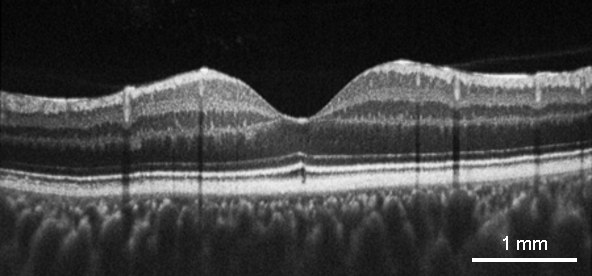
\includegraphics{figures/10_Introduction/oct.pdf}
      \caption{Transversal OCT image of the macula of a patient suffering from \textit{commotio retinae}\cite{Flatter2013}}
      \label{fig:OCTretina}
\end{figure}
The first implementations of these systems were restricted to side viewing, single modality OCT catheter-endoscopes that sampled the tissue by translating \cite{Feldchtein1998} or rotating \cite{Tearney1994} \cite{Tearney1996} the probe to acquire \textit{in-vivo} 2D cross sections through the lumen. This scanning method, displacing the entire catheter, resulted in poor dimmensional accuracy and speed. This can be solved by performing the scanning within the probe. Earlier works demonstrated this approach using Coherent Fiber Bundles (CFB) to create forward viewing endoscopes, where individual cores in the CFB were scanned sequentially to perform OCT imaging. The advantage of this method is that the scanning mechanism is located outside the body, which allows the endoscope tip to be relatively compact. As a tradeoff, the final image quality acquired with such systems suffer from poor SNR (signal-to-noise ratio) due to the CFB’s multi-mode behavior and distinct inter-core coupling \cite{Xie2005}. Furthermore, these systems are unsuitable for flexible endoscopes due to the rigidity of CFBs.

A new mechanism, the \textit{resonant fiber scanner} \cite{Seibel2001}, allowed forward-viewing video endoscopes with diameters under \SI{1}{\milli\meter} within thin, flexible catheters. An example of these systems is depicted in \autoref{fig:seibel}. They use the mechanical resonance of  a cantilever made of optical fiber to scan a laser at video speeds. Although this scanning method can be extended to confocal endomicroscopy \cite{Meinert}, it is challenging to implement OCT imaging, as it requires slower scanning speeds to allow the acquisition of the wavelength dependant information. Thus a method to lower the resonance frequency of the scanner is needed \cite{Huo2010}.

\begin{figure}[h!]\centering
      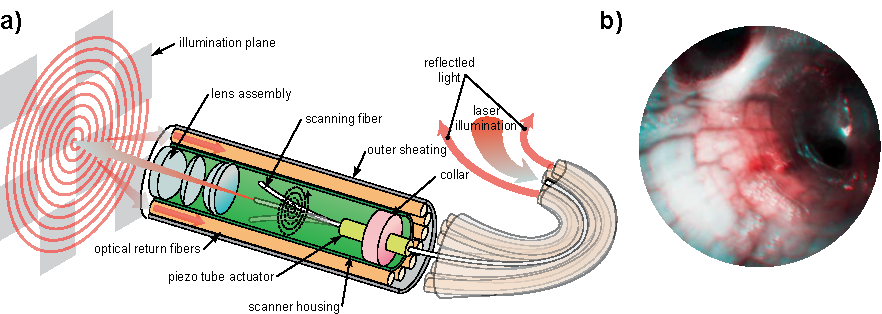
\includegraphics{figures/10_Introduction/seibel.pdf}
      \caption{\textbf{a)} Functional diagram of a resonant fiber scanner for video endoscopy with the scanning illumination fiber moving in a spiral scan pattern. \textbf{b)} Bronchoscopic image frames from standard RGB imaging at 500-line images at \SI{30}{\hertz} using the probe in a) \cite{Lee2010}.}
      \label{fig:seibel}
\end{figure}

With the advent of MEMS technology, it became possible to integrate active micro-mirrors on the distal side of the endoscope \cite{Liu2011}. The \emph{Gisela and Erwin Sick Chair for Microoptics} at the \emph{Institute for Microsystems Engineering} (IMTEK) has made recent advancements in the integration of different active scanning MEMS devices in microendoscopic probes, demonstrating OCT imaging \cite{Weber2012}.

Regarding the implementation of multi-modal endoscopic imaging systems, two major trends can be found in literature. The first of these is based on ultra-miniaturized fiber scanners and combines two confocal techniques, such as confocal laser microscopy, OCT and laser scanning fluorescence imaging \cite{Lorenser2013,Yoo2011}. However, the lack of full-field video-endoscopy hinders visual guidance during the endoscopic procedure. A commercial endoscope, with dimensions usually in the centimeter range, can be used in parallel, but, as each optical system has a different axis, it is difficult to correlate both images. The second approach uses a coherent fiber bundle (CFB) to image the tissue in white-light or narrow-band illumination, while individual cores in the CFB are scanned sequentially for the confocal imaging. But, as previously described, this approach is not well suited for OCT.

A third solution was developed at IMTEK within the HYAZYNT project \cite{Blattmann} \cite{Kretschmer} using a MEMS-based bimodal endoscopic probe which enable simultaneous full field imaging and OCT. The optical beampath of both modalities is combined before the objective lens, as depicted in \autoref{fig:hyazint}. The two imaging fields have the same optical axis, allowing for the registration of both images. Furthermore, the two-level design of the probe makes the integration of the two modalities possible while still decoupling their individual requirements. 
\begin{figure}[h!]\centering
      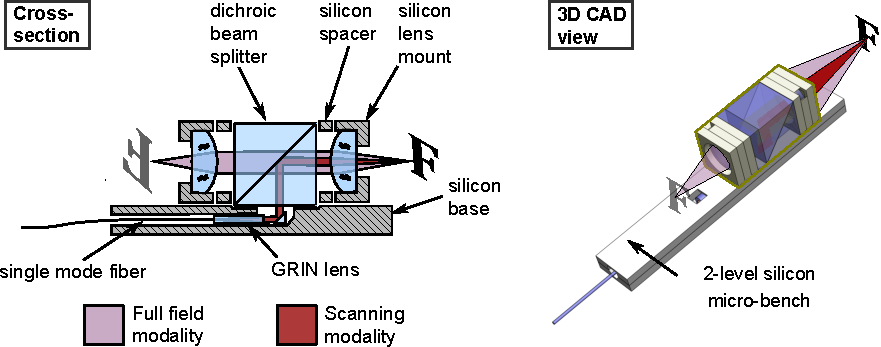
\includegraphics{figures/10_Introduction/hyazint.pdf}
      \caption{Schematic of the MEMS endomicroscope based on the HYAZINT probe \cite{Blattmann}. Two glass lenses at each side of a dichroic beamsplitter cube form the full field microscopy beam path. A silicon aperture is used to reduce the spherical aberrations. Buried beneath the full field optics, a single mode fiber glued to a collimating GRIN lens forms the OCT channel. A reflecting micro-prism glued to a dichroic beamsplitter cube combines the two beam paths.}
      \label{fig:hyazint}
\end{figure}
With the completion of the HYAZINT project, the OCT modality did not integrate a scanning mechanism to enable 3D imaging. Therefore, the aim of this work is to expand the concept demonstrated in the HYAZINT probe with the integration of a 2D fiber scanner optimized for OCT.


\section{Key results}
This thesis realizes a novel fiber scanner in a telecentric configuration which reduce the distortion in the OCT modality and enables its integration within a multi-modal probe with dimensions of $13 \times 2 \times \SI{3}{\milli\meter^3}$. The complete scanning engine has an outer diameter of \SI{0.9}{\milli\meter} and a length of \SI{9}{\milli\meter}, and features custom fabricated \SI{10}{\micro\meter} thick polyimide flexible interconnect lines to address the four piezoelectric electrodes. The small cross section of the probe combined with its short length enables its use in a wide gamut of lumens in form of flexible or tilting head endoscope.

A single modality probe was designed to independently investigate the performance of the OCT beampath. This probe, depicted in \autoref{fig:approachSketch}a, has an external diameter of \SI{2.5}{\milli\meter} and a total length of \SI{15}{\milli\meter}. Its optical design emulates that of the multimodal probe OCT path, enabling a direct translation of the results from this demonstrator probe to the multimodal one. To the best of our knowledge, this single modality probe is also one of the most compact implementation of an OCT microendoscope.

Using the demonstrator probe, it was possible to obtain preliminary \textit{en face} (\autoref{fig:approachSketch}b) and tomographic (\autoref{fig:approachSketch}c) images within a cylindrical volume of \SI{1}{\milli\meter} diameter and \SI{3}{\milli\meter} depth.

\begin{figure}[t]\centering
      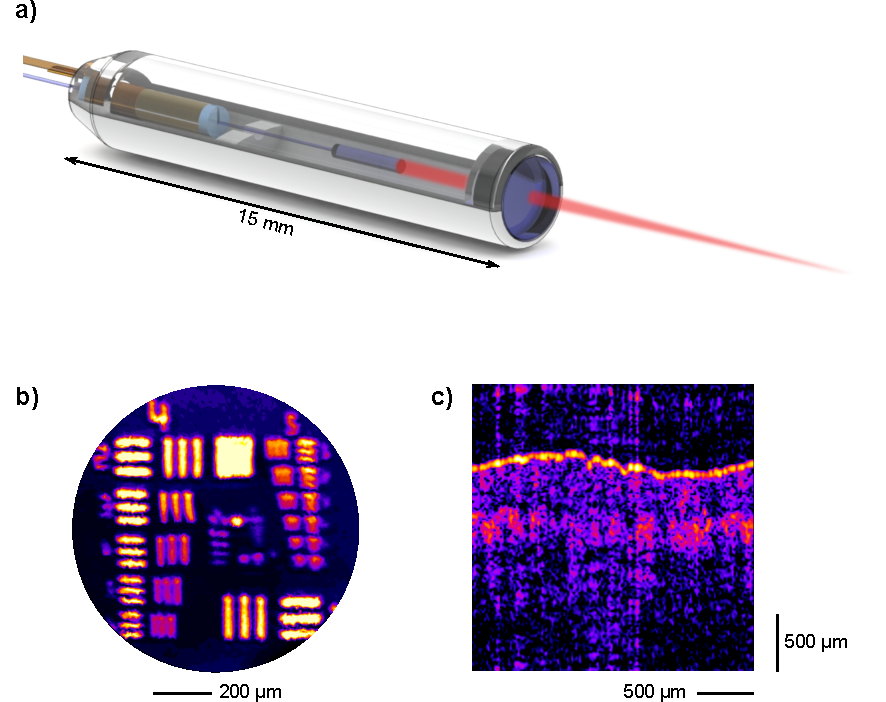
\includegraphics{figures/10_Introduction/summary.pdf}
      \caption{\textbf{a)} Render of the single modality demostrator.
      			\textbf{b)} \textit{En face} image of a chromium-on-glass test chart acquired using laser using the demonstrator probe.
      			\textbf{c)} OCT Image of a circular cross section of a human finger tip. Both images were obtained using the demonstrator probe.
      			}
      \label{fig:approachSketch}
\end{figure}